\documentclass[a4paper,titlepage]{scrartcl}
\pagestyle{plain}
\usepackage[utf8]{inputenc}
\usepackage[T1]{fontenc}
\usepackage[german]{babel}
\usepackage{float}
\usepackage{graphicx,tabularx}
\usepackage{amsmath,amssymb,amstext,mathabx}
\usepackage{enumerate}
\usepackage{units,longtable,subcaption}
\usepackage{mhchem, numprint,booktabs}
\usepackage[hidelinks]{hyperref}
\renewcommand{\sc}{\textsc}

\hypersetup{
    colorlinks,
    citecolor=black,
    filecolor=black,
    linkcolor=black,
    urlcolor=black
}

\numberwithin{equation}{section}

\title{Optische Pinzette}
\author{Genti Saliu\\Gruppe 106}
\date{Versuchstag: 26. Januar 2015}

\begin{document}
	\begin{titlepage}
		\maketitle
		\thispagestyle{empty}
	\end{titlepage}
	
\newpage
\pagenumbering{roman}
\tableofcontents

\newpage
\pagenumbering{arabic}

\section{Ziel des Versuchs}
In diesem Versuch wird gezeigt wie mikroskopische Objekte am Beispiel von Polystyrol-Kügelchen mit $\unit[3]{\mu m}$ Durchmesser mithilfe der optischen Pinzette von einem Ort auf einen anderen transportiert werden können.\\ \\
Weiterhin werden die Brownsche Bewegung der Kügelchen, die maximale Fangkraft der Pinzette und die Wahrscheinlichkeitsverteilung der Aufenthaltsorte der Kügelchen untersucht.
\section{Theoretische Grundlagen}
Die optische Pinzette (auf Englisch ''optical tweezer'') ist ein photonisches Gerät zum Festhalten (Einfangen) und Bewegen von Kolloiden (dielektrische Teilchen, die in einem Dispersionsmedium wie z.B. Gas oder Flüssigkeit fein verteilt sind). \cite{wiki:optischepinzette}\\ \\
Ihr Hauptbestandteil ist stark fokussierter Laserstrahl, der optische Kräfte erzeugt, mit denen sich Objekte der Größenordnung von $\unit[100]{\mu m}$ bis Atomgröße beliebig steuern lassen. Sie kommt in der künstlichen Befruchtung, zum Einfangen und Manipulation von biologischen Zellen, Viren, Bakterien und DNA zum Einsatz.
\subsection{Optische Kräfte}
Laserstrahlung mit gaußförmigen Intensitätsprofil wird durch eine Linse hoher numerischer Apertur (ein Objektiv) zu einem Punkt fokussiert. In diesem Punkt, der Fokuspunkt genannt wird und das Zentrum der optischen Falle darstellt, entsteht aufgrund dem senkrecht zur Ausbreitungsrichtung stehenden und gaußförmigen Intensitätsprofil ein harmonisches dreidimensionales Potential.\\ \\
Durch Richtungsänderung der einfallenden Photonen in der Probe entstehen optische Kräfte, die durch eine Impulsänderung $\Delta \vec{p}$ der Photonen aufgrund der Richtungsänderung verursacht werden. Aufgrund der Energieerhaltung erfährt nicht nur die einfallende Strahlung eine Impulsänderung, sondern auch das Objekt, an dem die Photonen ihre Richtung ändern:
\begin{equation*}
\vec{F}=\frac{\Delta \vec{p}}{\Delta T}
\end{equation*}
Bei der Beschreibung des Objektes in der optischen Falle muss zwischen zwei verschiedenen Kräften unterschieden werden. Zum einen die \emph{Streukraft}, die das Objekt in Ausbreitungsrichtung des Strahls transportiert und vom Photonendruck herrührt. Dabei werden Photonen überwiegend zurück zum Laser reflektiert. Diese Kraft destabilisiert die Falle und muss von der zweiten Kraft, die \emph{Gradientenkraft}, überkompensiert werden. Aufgrund der Fokussierung entsteht in der Nähe des Fokuspunktes ein starker Intensitätsgradient, die zu einer Kraft führt, die in Richtung der höchsten Intensität, dem Fokuspunkt, gerichtet ist.\\ \\
Die erste Untersuchung dieser durch Strahlungsdruck des Lichtes entstehenden Kräfte auf mikroskopische Teilchen gelang 1970 dem Experimentalphysiker Arthur Ashkin in seinem Paper ''Acceleration and trapping of particles by radiation pressure'' \cite{ashkin1970}. Bis dahin war dies aufgrund von thermischen Einflüssen, die durch Temperaturgradienten im umgebenden Medium verursacht wurden, nicht möglich gewesen. Diese sogenannten radiometrischen Effekte erzeugten Kräfte um Größenordnungen größer als die des Strahlungdrucks. Ashkin besetigte sie, indem er transparente Teilchen (Latexkügelchen) in einem transparenten Medium (Wasser) suspendierte.\\ \\
Um das Zustandekommen der optischen Kräfte zu beschreiben, werden wir das Objekt kugelförmig annehmen. Dabei sind je nach Kolloidengröße drei Fälle zu unterscheiden:
\begin{itemize}
\item Rayleigh-Regime ($2R_K \ll \lambda$) - die zu fangenden Objekte sind viel kleiner als die Wellenlänge des Laserstrahls. Deshalb nähert man das Teilchen durch einen Punktdipol und nutzt dabei die elektromagnetische Natur des Lichts.
\item Übergangsregime ($2R_K \approx \lambda$) - dieser stellt einen Übergangsbereich zwischen Rayleigh- und Mie-Regime dar und wird in diesem Protokoll nicht behandelt.
\item Mie-Regime ($2R_K \gg \lambda$) - in diesem Fall kann die geometrische Optik zur Beschreibung der auftretenden Kräfte verwendet werden.
\end{itemize}
\subsubsection{Mie-Regime}
Zur Entstehung der optischen Kräfte wird hier die geometrische Optik verwendet. Dazu ist das einfallende Laserlicht als viele einzelne Lichtstrahlen, die sich geradlinig in einem homogenen Medium ausbreiten, zu betrachten. Beugungserscheinigung treten aufgrund der Behandlung durch die geometrische Strahlenoptik nicht auf. Die optischen Kräfte entstehen aufgrund der Brechung der Lichtstrahlen an Medien mit verschiedenen Brechungsindizes.\\ \\
Man ordne den Teilchen einen Brechungsindex $n_2$ und dem umgebenden Medium einen Brechungsindex $n_1$ zu. Der Strahl besitzt einen Impuls $\vec{p}$ proportional zur Energie und Ausbreitungsrichtung. Fällt nun ein Strahl $r_m$ auf das Objekt ein (Abbildung \ref{fig:strahlen}), so wird ein Teil reflektiert ($r_{m_1}$) während der andere Teil transmittiert und an den Grenzflächen der Kugel gebrochen wird.
\begin{figure}[H]
	\centering
	\begin{tabular}{@{}r@{}}
		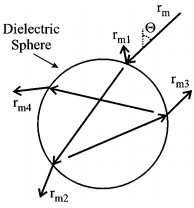
\includegraphics[width=0.25\textwidth]{strahlen.PNG}\\
		\footnotesize\sffamily\textbf{Quelle:} Artikel \cite{smith1999}, Seite 27
	\end{tabular}
	\caption{Diagramm mit auf einer dielektrischen Kugel einfallendem Strahl $r_m$, reflektiertem Strahl $r_{m_1}$ und gebrochenen Strahlen $r_{m_2}$, $r_{m_3}$ und $r_{m_4}$}
    \label{fig:strahlen}
\end{figure}
Dabei ändert sich der Impuls des Strahls um $\Delta \vec{p}$, was nach dem Impulserhaltungsgesetz eine Impulsänderung der Kugel um den gleichen Betrag bewirkt. Insgesamt wirkt auf die Kugel eine Kraft $\vec{F}$, die sich in Streu- und Gradientenkraft (Abbildung \ref{fig:streugradient}) aufteilen lässt:
\begin{description}
\item[Streukraft:] diese Kraft wirkt in Einfallsrichtung des Laserstrahls und entsteht durch Reflektion des Strahls an Strahlein- und Strahlaustrittsfläche. Die Kugel wird in Strahlrichtung beschleunigt. Diese Kraft soll möglichst minimiert werden.
\item[Gradientenkraft:] die Gradientenkraft wirkt in Richtung des Intensitätsmaximums entlang des Intensitätsgradienten, in der Richtung aus der Lichtstrahl eintrifft. Diese Kraft bewirkt das Einfangen des Teilchens und sollte deshalb möglichst maximiert werden.
\end{description}
\begin{figure}[H]
	\centering
	\begin{tabular}{@{}r@{}}
		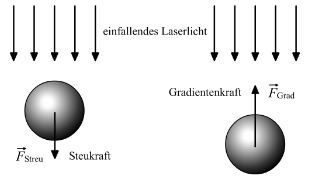
\includegraphics[width=0.5\textwidth]{streugradientenkraft.png}\\
		\footnotesize\sffamily\textbf{Quelle:} Praktikumsprotokoll \cite{protokoll}
	\end{tabular}
	\caption{Streu- und Gradientenkräfte}
    \label{fig:streugradient}
\end{figure}
Nun werden wir die beiden Kräfte, die ein unter dem Winkel $\theta$ einfallender Lichtstrahl der Intensität $P$ auf das kugelförmige Teilchen ausübt, berechnen. Dem Lichtstrahl wird ein Impuls $p$ zugeordnet:
\begin{equation*}
p=\frac{n_1 P}{c}
\end{equation*}
wobei $c$ die Lichtgeschwindigkeit im Vakuum ist. Den Anteil reflektierter und transmittierter Leistung bestimmt man anhand der Fresnelschen Reflektions- und Transmissionskoeffizienten $R$ und $T$:
\begin{align*}
R&=\frac{I_r \cos{\theta_r}}{I_e \cos{\theta_e}}=\left( \frac{n_1-n_2}{n_1+n_2} \right)^2\\
T&=\frac{I_t \cos{\theta_t}}{I_e \cos{\theta_e}}=\left( \frac{2n_1}{n_1+n_2} \right)^2
\end{align*}
Dabei sind $I_r$ die reflektierte Intensität, $I_e$ die Intensität des Einfallstrahls, $I_t$ die Intensität des transmittierten Strahls, $\theta_r$, $\theta_e$ und $\theta_t$ jeweils der Reflektions-, Einfalls- und Transmissionswinkel. Ausserdem gilt für den Einfall- und Reflektionswinkel $\theta_e=\theta_r$.\\ \\
Weil Brechung und Transmission mehrmals auftreten können, werden die Impulse für alle Brechungs- und Transmissionsmöglichkeiten beim Übergang des Lichtstrahls vom Medium in die Teilchen aufsummiert. Vor einem Übergang beträgt die Summe $p=\frac{n_1 P}{c}$ für die Streukraft und $0$ für die Gradientenkraft. Wir stellen deshalb für die Streu- und Gradientenkraft folgende Lösungen in Abhängigkeit des Einfallwinkels $\theta_e$:
\begin{align*}
F_{Streu}(\theta_e)&=\frac{n_1 P}{c} \left( 1 + R \cos{(2 \theta_e)} - \frac{T^2 (\cos{(2 \theta_e - \theta_t)} + R \cos{(2 \theta_e)})}{1+R^2+2R\cos{(2 \theta_t)}} \right)\\
F_{Grad}(\theta_e)&=\frac{n_1 P}{c} \left( R \sin{(2 \theta_e)} - \frac{T^2 (\sin{(2 \theta_e-\theta_t)} + R \sin{(2 \theta_e)})}{1+R^2+2R\cos{(2 \theta_t)}} \right)
\end{align*}
Damit das Teilchen im Strahlengang eingefangen werden kann, muss die Gradientenkraft also größer als die Streukraft für alle unter verschiedenen Winkeln $\theta_e$ einfallenden Strahlen sein. Zur Vereinfachung der Kräftegleichungen führen wir den Gütefaktor $Q$ ein:
\begin{align*}
F_{Streu}(\theta_e)&=Q_{Streu}(\theta_e) \cdot \frac{n_1 P}{c}\\
F_{Grad}(\theta_e)&=Q_{Grad}(\theta_e) \cdot \frac{n_1 P}{c}
\end{align*}
Abbildung \ref{fig:guetefaktor} zeigt den Verlauf der Streu- und Gradientenkräfte für Einfallswinkel $\unit[0]{^\circ}$ bis $\unit[90]{^\circ}$. Darin ist zu erkennen, wie die Lichtstrahlen für einen Winkel $\approx \unit[70]{^\circ}$ die größte Gradientenkraft besitzen, d.h. Lichtstrahlen müssen in möglichst großen Winkeln im $\unit[70]{^\circ}$-Bereich eingestrahlt werden.
\begin{figure}[H]
	\centering
	\begin{tabular}{@{}r@{}}
		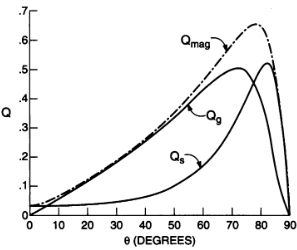
\includegraphics[width=0.5\textwidth]{guetefaktor.png}\\
		\footnotesize\sffamily\textbf{Quelle:} Artikel \cite{ashkin1992}
	\end{tabular}
	\caption{Beträge von Streu- und Gradientenkraft zur Gesamtkraft in Abhängigkeit vom Einfallswinkel $\theta_e$}
    \label{fig:guetefaktor}
\end{figure}
\subsubsection{Rayleigh-Regime}
Im Rayleigh-Regime, die wir hier nur kurz aufgreifen, ist der Teilchendurchmesser $2R_K$ viel kleiner als die Wellenlänge des eingestrahlten Lichts und das Teilchen wird deshalb als Punktdipol angesehen.\\ \\
Das Teilchen besitze wieder einen Brechungsindex $n_2$ und das umgebende Medium einen Brechungsindex $n_1$. Sei ausserdem $m=\frac{n_2}{n_1}$ der relative Brechungsindex und $k=\frac{2 \pi n_1}{\lambda}$ der Wellenvektor des Lichtstrahls. Für die Kräfte gilt dann:
\begin{description}
\item[Die Streukraft] ist proportional zum Energiefluss und zeigt in Richtung des einfallenden Lichtstrahls:
\begin{equation*}
\vec{F}_{Streu}=n_1 \frac{\langle \vec{S} \rangle \sigma}{c} \quad \quad \text{mit} \quad \quad \sigma=\frac{8}{3} \pi (kr)^4r^2 \left( \frac{m^2-1}{m^2+2} \right)^2
\end{equation*}
wobei $\sigma$ der Wirkungsquerschnitt des Teilchens mit Radius $r$ und $\langle \vec{S} \rangle$ der zeitliche Mittelwert des Poynting-Vektors sind.
\item[Die Gradientenkraft] im Rayleigh-Regime ist proportional und parallel zum Gradienten der Energiedichte:
\begin{equation*}
\vec{F}_{Grad}=\frac{\alpha}{2} \nabla \langle \vec{E}^2 \rangle \quad \quad \text{mit} \quad \quad \alpha=n_1^2r^3 \left( \frac{m^2-1}{m^2+2} \right)^2
\end{equation*}
wobei $\alpha$ die Polarisierbarkeit des Teilchens und $\langle \vec{E}^2 \rangle$ der zeitliche Mittelwert des Energiequadrates sind.
\end{description}
Diese Ergebnisse fassen wir zu einem Gütefaktor zusammen:
\begin{equation*}
Q=\frac{F_{Grad}}{F_{Streu}}=\frac{3 \sqrt{3} \cdot n_1^2 \cdot \lambda^5 \cdot (m^2 + 2)}{64 \pi^5 \cdot (m^2-1) \cdot r^2 \omega_0^2}
\end{equation*}
Dabei muss für den Gütefaktor $Q \gg 1$ gelten, also die Gradientenkraft muss die Streukraft erheblich überwiegen.\\ \\
Abbildung \ref{fig:rayleigh} zeigt die Verlauf der Lichtstrahlen im Fokus. Dabei ist die Strahlentaille $\omega_0$ der Radius der Fokus, in dem sich das gefangene Objekt befindet.
\begin{figure}[H]
	\centering
	\begin{tabular}{@{}r@{}}
		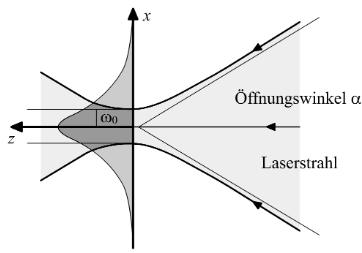
\includegraphics[width=0.5\textwidth]{rayleigh.png}\\
		\footnotesize\sffamily\textbf{Quelle:} Praktikumsprotokoll \cite{protokoll}
	\end{tabular}
	\caption{Lichtstrahlen im Fokus}
    \label{fig:rayleigh}
\end{figure}
Für die Strahlentaille $\omega_0$ gilt:
\begin{equation*}
\omega_0=\frac{\lambda}{\pi \cdot NA}
\end{equation*}
wobei $NA$ die numerische Apertur des Objektivs ist. Die numerische Apertur $NA$ bezeichnet das Vermögen eines optischen Elements, Licht zu fokussieren, also den Umfang an Winkeln, mit denen Licht ins System eindringen oder vom System emittiert werden kann. Sie ergibt sich aus dem Produkt vom Brechungsindex $n$ des Materials zwischen Objektiv und Fokus und dem Sinus des halben objektseitigen Öffnungswinkels $\alpha$:
\begin{equation*}
NA=n\cdot \sin \alpha
\end{equation*}
\subsection{Brownsche Bewegung}
Die Brownsche Bewegung beschreibt die unregelmäßige und ruckartige Wärmebewegung kleiner, mikroskopisch sichtbaren Teilchen in Flüssigkeiten und Gasen. Dabei stoßen diese Teilchen ständig mit den Teilchen einer Flüssigkeit. Die mikroskopischen Teilchen legen einen Weg zurück, der der mittleren freien Weglänge entspricht. Danach findet wieder ein Stoß mit Flüssigkeitsteilchen und das Teilchen beschreibt einen neuen Weg.\\ \\
Aufgrund der Temperatur $T$ besitzen die Teilchen eine mittlere kinetische Energie $\overline{E}$:
\begin{equation*}
\overline{E}=\frac{3}{2}k_BT
\end{equation*}
wobei $k_B$ die Boltzmann-Konstante ist. Aufgrund dieser thermischen Energie bewegen sich die Teilchen mit der mittleren thermischen Geschwindigkeit $\overline{v}$:
\begin{align*}
\overline{E}=&\frac{3}{2}k_BT=\frac{m\overline{v}^2}{2}\Rightarrow \\
\overline{v}=&\sqrt{\frac{3k_BT}{m}}
\end{align*}
Demnach besitzen schwere Teilchen eine geringere mittlere Geschwindigkeit als leichtere. Die Brownsche Bewegung kann sich leicht mit einem Mikroskopen beobachten lassen.\\ \\
Zur Auswertung der Brownschen Bewegung verwendet man die mittlere quadratische Verschiebung. Für ein Teilchen mit Anfangsposition $(x(0),y(0))$ beträgt die Verschiebung zur Zeit $t_i$:
\begin{equation}
\label{eq:verschiebungEinfach}
r^2(t_i)=(x(t_i)-x(0))^2+(y(t_i)-y(0))^2
\end{equation}
Die mittlere quadratische Verschiebung bis zur Zeit $t_n$ beträgt:
\begin{equation*}
\langle r^2 \rangle_{time}(t_n)=\frac{1}{n} \sum_{i=1}^{n} r^2(t_i)
\end{equation*}
Um Abweichungen aufgrund von möglichen Ausreißern für bestimmte Teilchen zu minimieren, wird der Mittelwert über mehrere Partikel $M$ gebildet:
\begin{equation}
\label{eq:verschiebung}
\langle r^2 \rangle_{time}(t_n)=\frac{1}{M} \sum\left( \frac{1}{n} \sum_{i=1}^{n} r^2(t_i) \right)
\end{equation}
Für die mittlere quadratische Verschiebung in zwei Dimensionen gilt:
\begin{equation}
\langle r^2(t) \rangle=\overline{v}lt=4Dt
\label{eq:dmsDiffusion}
\end{equation}
wobei für die Diffusionskonstante $D$ laut der Einsteinschen Relation gilt:
\begin{equation}
D=\frac{k_bT}{6\pi \eta a}
\label{eq:diffusionskonstante}
\end{equation}
Dabei sind $\eta$ die Viskosität der umgebenden Flüssigkeit und $a$ der Teilchenradius. Man sieht leicht, dass die mittlere quadratische Verschiebung proportional mit der Zeit anwächst.\\ \\
Die Viskosität $\eta$ lässt sich anhand obiger Formeln bestimmen, wenn man die mittlere quadratische Verschiebung pro Zeit $m=\frac{\langle r^2(t) \rangle}{t}$ kennt:
\begin{equation*}
\eta=\frac{2k_BT}{3 \pi a m}
\end{equation*}
\subsection{Reibungskraft einer laminaren Flüssigkeit}
Auf eine Kugel mit Radius $a$, die sich in eine Lösungsflüssigkeit mit Viskosität $\eta$ mit der Geschwindigkeit $v$ bewegt, wirkt für eine laminare Umströmung die Stokesche Reibungskraft $F_{Stokes}$:
\begin{equation*}
F_{Stokes}=6 \pi \eta a v
\end{equation*}
So wirkt auf die sich in der optischen Falle befindlichen Kugel, außer der optischen Kraft $F_T$, auch die obige Reibungskraft $F_{Stokes}$.\\\\
Bezeichnet man mit $v_{max}$ die maximale Geschwindigkeit, die die Kugel aufgrund der optischen Kraft der Pinzette erreichen kann, so wird sie noch in der Falle gehalten, falls gilt:
\begin{equation*}
F_T=F_{Stokes}
\end{equation*}
Somit kann man durch die Messung der maximalen Geschwindigkeit $v_{max}$ die maximale Fangkraft der optischen Pinzette $F_T$ bestimmen:
\begin{equation}
F_T=6 \pi \eta a v_{max}
\label{eq:fangkraft}
\end{equation}
Die Fangkraft der Pinzette $F_T$ hängt offensichtlich nicht von der Masse der Kugel ab.
\section{Experimenteller Aufbau}
Die optische Pinzette besteht im Wesentlichen aus zwei Komponenten: einem \emph{Lasersystem} zum Einfangen und Verschieben kleiner Teilchen und einem \emph{optischen Mikroskopen} zur Beobachtung der Kolloiden und Verschiebungsvorganges.
\begin{figure}[H]
\begin{minipage}{.5\textwidth}
\centering
\begin{tabular}{@{}r@{}}
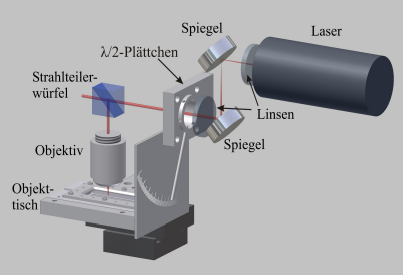
\includegraphics[width=0.8\textwidth]{pinzette.PNG}\\
\footnotesize\sffamily\textbf{Quelle:} Praktikumsvorbereitung Uni Stuttgart \cite{praktikum}
\end{tabular}
\caption{Optische Pinzette}
\label{fig:pinzette}
\end{minipage}
\begin{minipage}{.5\textwidth}
\centering
\begin{tabular}{@{}r@{}}
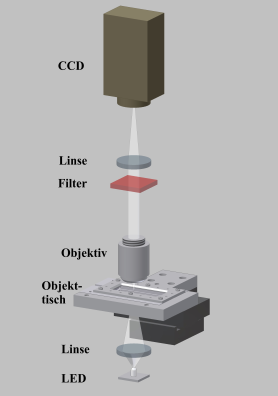
\includegraphics[width=0.7\textwidth]{mikroskop.PNG}\\
\footnotesize\sffamily\textbf{Quelle:} Praktikumsvorbereitung Uni Stuttgart \cite{praktikum}
\end{tabular}
\caption{Mikroskop}
\label{fig:mikroskop}
\end{minipage}
\end{figure}
Das \emph{Lasersystem} (Abbildung \ref{fig:pinzette}) besteht aus einem Diodenlaser mit Wellenlänge $\lambda=\unit[638]{nm}$, der mithilfe von zwei Spiegeln so aufgeweitet wird, dass das Objektiv möglichst vollständig ausgeleuchtet ist. Die erste Linse hat eine Brennweite von $f_1=\unit[5]{cm}$, die zweite ist in einem Abstand entsprechend ihrer Brennweite von $f_2=\unit[20]{cm}$ hinter dem Fokuspunkt des Lasers positioniert. Je größer die benötigte Aufweitung, umso größer soll die Differenz der Brennweiten der Linsen $f_2-f_1$ sein.
\begin{figure}[H]
	\centering
	\begin{tabular}{@{}r@{}}
		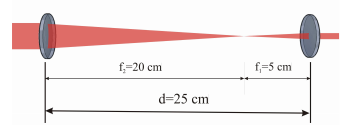
\includegraphics[width=0.5\textwidth]{twolenses.PNG}\\
		\footnotesize\sffamily\textbf{Quelle:} Vorbereitungsmappe \cite{vorbereitungsmappe}
	\end{tabular}
	\caption{Aufweitung des Strahls durch 2 Linsen}
    \label{fig:twolenses}
\end{figure}
Danach trifft der aufgeweitete Strahl auf einen Strahlenteiler, der den Laserstrahl auf das Objektiv mit numerischer Apertur 8.5 und auf die Probe lenkt. Dabei wird nur $\unit[8.1]{mW}$ von den $\unit[25]{mW}$ an Laserleistung auf das Objektiv reflektiert. Unter Verwendung zweier Servomotoren kann die Probe auf dem Objekttisch in $x$- und $y$-Richtung bewegt werden, dadurch wird die Bewegung des Lasers relativ zur Probe und damit eine Verschiebung der Teilchen in der Probe verursacht.\\ \\
Das \emph{Mikroskop} (Abbildung \ref{fig:mikroskop}) dient der Betrachtung der Probe auf dem PC. Die Probe wird zur besseren Beobachtung von unten durch eine LED-Lampe belichtet, deren Lichstrahlen mit einer Linse aufgeweitet werden. Oberhalb des Strahlenteilers der Pinzette befindet sich eine CCD-Kamera, die vor Überbelichtung durch zwei Rotfilter geschützt ist und ein Abbild der Probe aufnimmt. Durch die Einstellung des Abstands zwischen Probe und Objektiv mit einer Mikrometerschraube kann das Probenabbild justiert werden.\\ \\
Mit einem Durchmesser $2R_K=\unit[3 \cdot 10^{-6}]{m}$ für die Kolloide und eine Wellenlänge $\lambda=\unit[0.638 \cdot 10^{-6}]{m}$ für den Laserstrahl, sind die optischen Kräfte mithilfe des Mie-Regimes ($2R_K \gg \lambda$) zu erklären.
\section{Durchführung des Versuchs}
\subsection{Vorbereitung}
Mithilfe des Assistenten wurden der PC, die optische Pinzette und Mikroskop im Betrieb genommen. Dann war der Objekttisch des Mikroskops mithilfe der Mikrometerschraube auf die CCD-Kamera zu fokussieren, sodass die Kolloide auf dem Computerbildschirm gut zu erkennen waren.\\ \\
Dazu stellten wir zunächst die Probe her. Wir verwendeten Polystyrol-Kügelchen mit einem Durchmesser von $\unit[3]{\mu m}$. Zunächst spritzten wir sie in den Probebehälter ein.
Da die Kügelchen in sehr konzentrierter Form vorhanden waren und somit für den Versuch ungeeignet, verdünnten wir die Lösung mit destilliertem Wasser, indem wir dort eine kleine Menge einspritzten. Mithilfe der Spritzdüse wurde die Lösung durchmischt.\\ \\
Anschließend erfolgte die Fokussierung des Objektträgers nach der Vorschrift der Vorbereitungsmappe durch den Assistenten. Auf dem Bildschirm war nach erfolgreicher Fokussierung das Bild in Abbildung \ref{fig:laboraufnahme1} zu sehen.
\begin{figure}[H]
	\centering
	\begin{tabular}{@{}r@{}}
		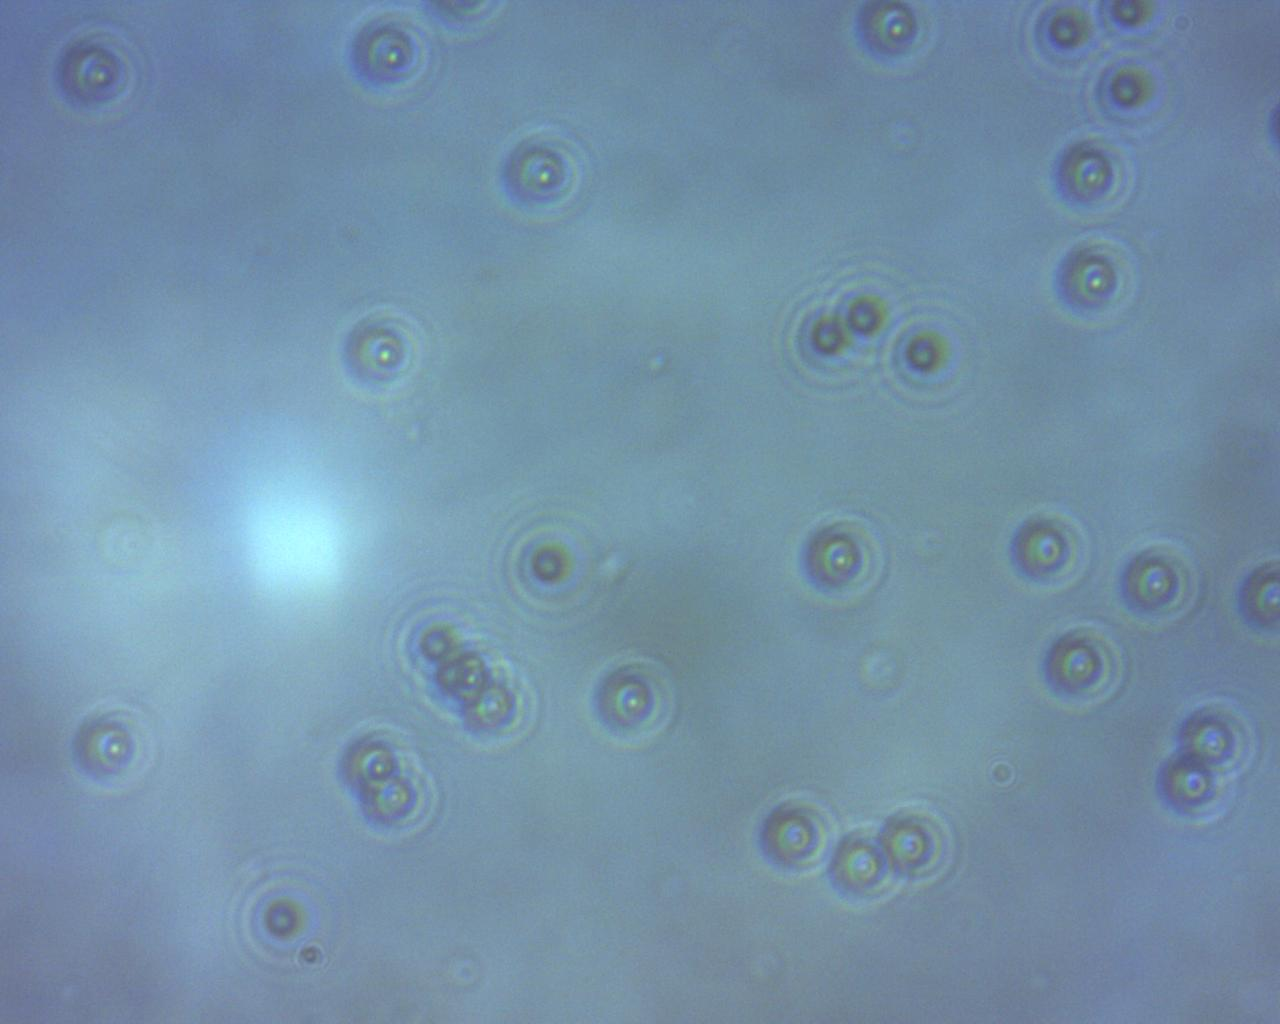
\includegraphics[width=0.37\textwidth]{aufgabe3-2.jpg}\\
		\footnotesize\sffamily\textbf{Quelle:} Laboraufnahme
	\end{tabular}
	\caption{Polystyren-Kügelchen im Mikrosokop}
    \label{fig:laboraufnahme1}
\end{figure}
\subsection{Anordnung von Polystyren-Kügelchen}
In diesem Versuchsteil verwendeten wir Polystyren-Kügelchen vom Durchmesser $\unit[3]{\mu m}$ und versuchten mithilfe der optischen Pinzette so viele wie möglich davon an einem Ort zu verschieben (Abbildung \ref{fig:laboraufnahme3}). Dabei konnten wir die Bewegungsgeschwindigkeit mit den Servomotoren ansteuern.
\begin{figure}[H]
	\centering
	\begin{tabular}{@{}r@{}}
		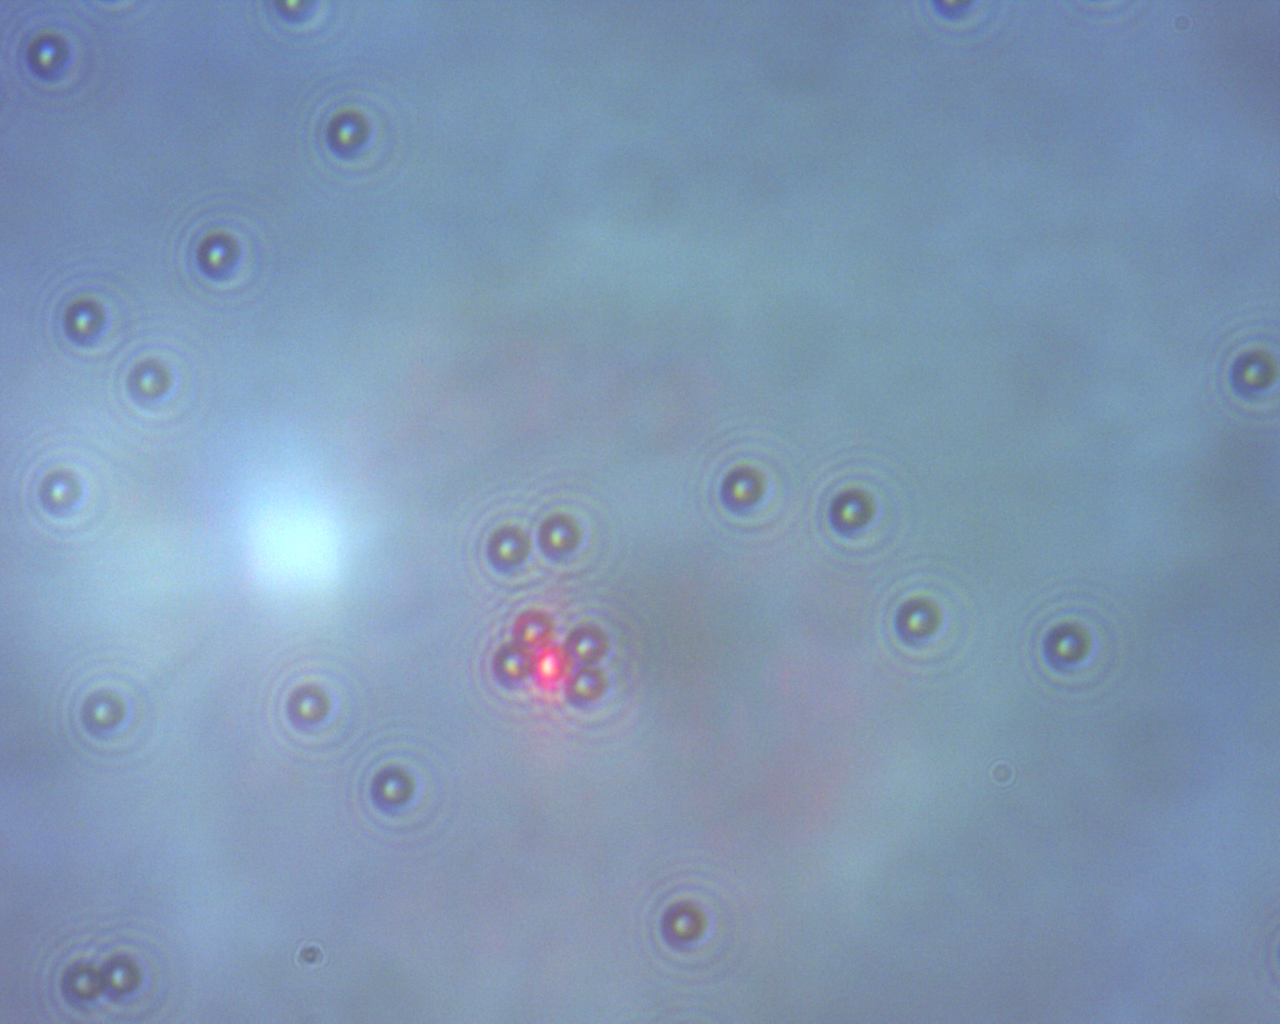
\includegraphics[width=0.37\textwidth]{teilchengruppe.png}\\
		\footnotesize\sffamily\textbf{Quelle:} Laboraufnahme
	\end{tabular}
	\caption{An einem Ort verschobene Kügelchen}
    \label{fig:laboraufnahme3}
\end{figure}
Hier ging es vor allem darum sich von der optischen Pinzette zu überzeugen und sich mit der Bedienung vertraut zu machen.
\subsection{Seife als klassisches Beispiel von Fett}
Mangels Fettlösungen wurde dieser Versuchsteil nicht durchgeführt.
\subsection{Untersuchung von Schimmel mit der optischen Pinzette}
Mangels Schimmellösungen wurde dieser Versuchsteil nicht durchgeführt.
\subsection{Fangkraft}
\subsubsection{Brownsche Bewegung}
In diesem Versuchsteil sollte die Brownsche Bewegung von Teilchen beobachtet werden. Eine echte Brownsche Bewegung konnten wir aufgrund der Driftbewegung der Teilchen nicht beobachten, obwohl wir mehrere Proben herstellten und untersuchten.\\ \\
Nach mehreren Versuchen gelang es uns eine Probe aufzubereiten, bei der die Driftgeschwindigkeit sehr klein erschien und die Bewegung der Kolloiden die aus der Brownschen Bewegung bekannte Unregelmäßigkeit aufzuweisen schien. Danach erfolgte eine 2-minütige Videoaufnahme der Probe. Anschließend suchten wir uns 5 passende Partikeln aus und messten aus der Videodatei für jedes die Aufenthaltsorte zu unterschiedlichen Zeiten mithilfe der im Labor zur Verfügung stehenden Software.
\subsubsection{Maximale Fangkraft}
Wie aus der Vorbereitung bekannt, muss zur Bestimmung der maximalen Fangkraft die maximale Geschwindigkeit $v_{max}$ bekannt sein. Dies wurde im Labor zu $v_{max}=\unit[0.06]{\frac{mm}{s}}$ gemessen.\\ \\
Um sie zu messen, bewegten wir ein gefangenes Kügelchen mit der größtmöglichen Geschwindigkeit, bei der sich das Teilchen noch in der optischen Falle gefangen bleiben konnte und stellten die Zeit und den zurückgelegten Weg fest.\\\\
Da das Programm den Weg in Pixels angezeigt hat, musste zusätzlich eine Kalibrierungsmessung gemacht werden, um Pixels in Millimetern zu konvertieren. Die Anzeige des Mikroskopbilds auf dem Bildschirm erfolgte in einer Auflösung von $1280$ Pixelbreite und $1024$ Pixelhöhe.\\ \\
Dazu wurde ein im Laserstrahl eingefangenes Teilchen benutzt. Sie wurde zunächst an den linken Rand des Bildschirms gefahren. Dort lasen wir die Positionsangabe auf der $x$-Achse $x_{links}=\unit[0.1748]{mm}$ aus der Anzeige in roten Ziffern des Servomotors ab. Dann bewegten wir das Teilchen an den rechten Rand und lasen erneut die Positionsangabe auf der $x$-Achse $x_{rechts}=\unit[0.2964]{mm}$ ab. Die Differenz dieser Positionsangaben entspricht dem Abstand vom linken zum rechten Rand. Daraus erhalten wir welchem Abstand 1 Pixel auf dem Bildschirm entspricht (Kalibrierungsfaktor $k$):
\begin{equation*}
k=\frac{\unit[(0.2964 - 0.1748) \cdot 10^{-3}]{m}}{\unit[1280]{px}}=\unit[0.095]{\frac{\mu m}{px}}
\end{equation*}
\subsection{Wahrscheinlichkeitsverteilung der Aufenthaltsorte der Teilchen}
In diesem Teil war die Wahrscheinlichkeitsverteilung der Aufenthaltsorte eines freien und gefangenen Teilchen zu bestimmen. Es wird eine Maxwell-Boltzmann-Verteilung erwartet, jedoch muss diese anhand der Messdaten bestätigt oder wiederlegt werden.\\ \\
Die Strahlleistung war auf $\unit[3]{mW}$ zu reduzieren. Wir führten eine 4-minütige Videoaufnahme eines freien und eines mit der Pinzette gefangenen Teilchens durch, die im Anschluss mit Software ausgewertet wurde, indem für die beiden Teilchen die Aufenthaltsorte zu verschiedenen Zeiten des Videos gemessen und als TSV (Tab Separated Values)-Datei gespeichert wurden.
\subsection{Farbstoffe im Brennpunkt des Lasers}
Dieser Teil beschäftigte sich mit einem qualitativen Experiment: man sollte beobachten, wie sich Farbmoleküle aus einem Markierstift unter dem Einfluss der Laserlichts verhalten. Die Farbmoleküle befinden sich in einer Ethanollösung.\\ \\
Dabei färbten wir den Objektträger des Mikroskops zunächst rot und dann schwarz ein und verdünnten jedes Mal die Farbe mit distilliertem Wasser.\\ \\
Als der Laserstrahl auf den rot-gefärbten Objektträger auftraff, wurde die rote Farbe verstärkt, d.h. der Großteil des Strahles wurde reflektiert - sehr wenig wurde transmittiert. Die Haltekraft des Laserstrahls ist aufgrund des kleinen Impulses gering.\\ \\
Bei der schwarzen Farbe (Abbildung \ref{fig:laboraufnahme2}) trat das Gegenteil auf: die Stelle, wo der Laserstrahl eintraf, wurde weiß, d.h. das sichtbare Licht wurde komplett absorbiert, die Farbmoleküle wurden durch die Absorption erhitzt und aufgelöst. Der Laser wirkte in diesem Fall destruktiv.
\begin{figure}[H]
	\centering
	\begin{tabular}{@{}r@{}}
		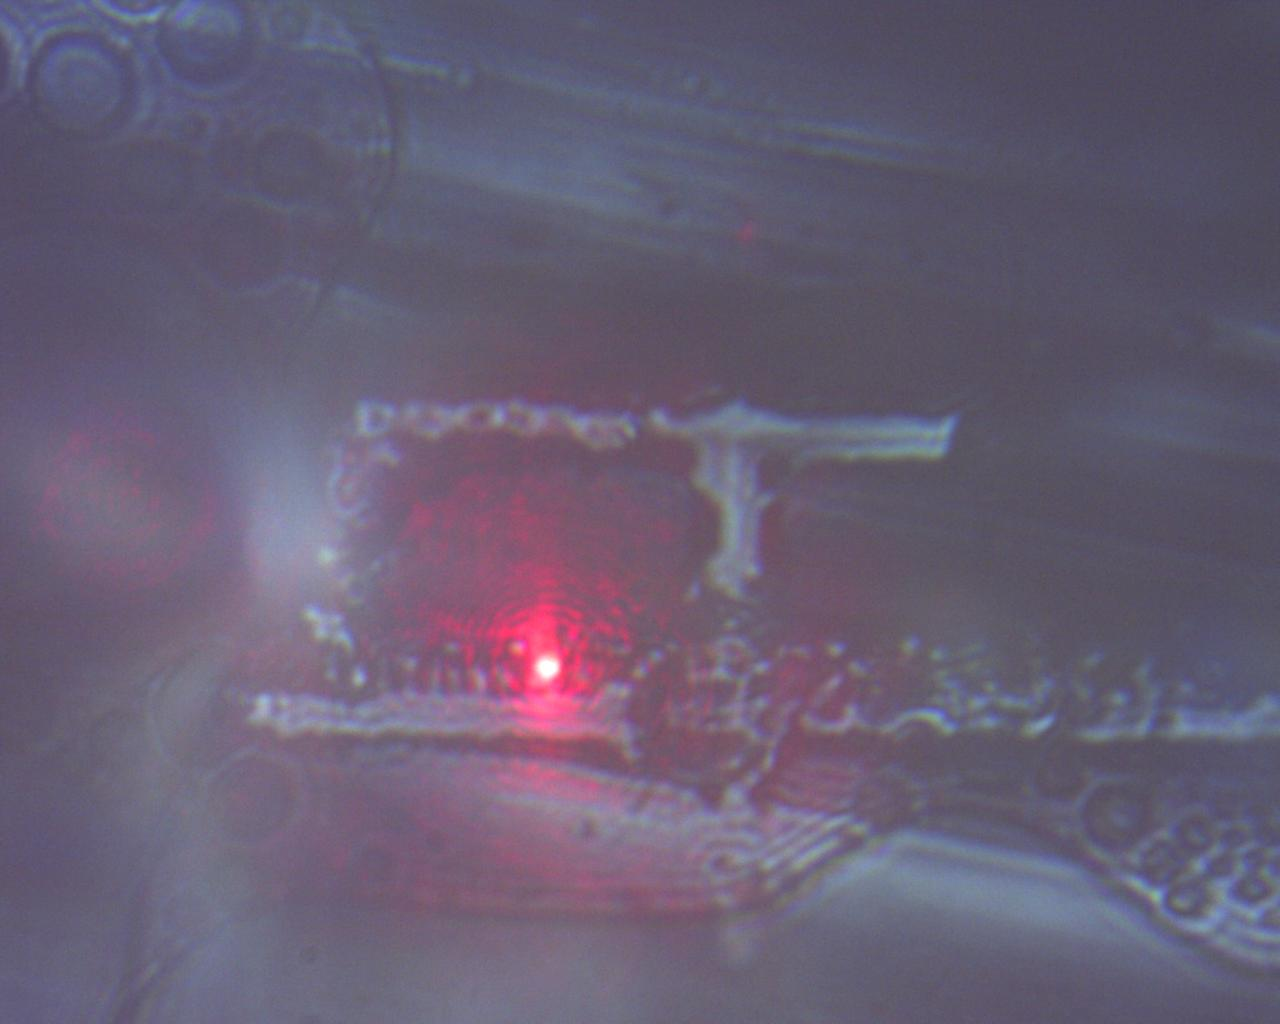
\includegraphics[width=0.2\textwidth]{aufgabe3-7-schwarz.jpg}\\
		\footnotesize\sffamily\textbf{Quelle:} Laboraufnahme
	\end{tabular}
	\caption{Laserstrahlengang auf schwarz-gefärbtem Objektträger}
    \label{fig:laboraufnahme2}
\end{figure}
Eine mögliche Anwendung dieser Phänomene ist das Matrix-Schreiben auf Oberflächen: man überzieht den Teil der Oberfläche, der nicht bearbeitet werden soll, mit einer reflektierenden Schicht und den Teil der Oberfläche, der ''beschriftet'' werden soll mit einer absorbierenden Schicht. Bestrahlt man die gesamte Oberfläche durch Laserlicht, erhält man das gewünschte Muster.\\ \\
Bei roter Farbe induziert der Laser, sofern er indestruktiv absorbiert wird, Fluoreszenz.
\section{Auswertung}
\label{subsec:brown}
\subsection{Brownsche Bewegung}
Wir trugen die mittlere quadratische Verschiebung gegen die Zeit in einem Diagram auf (Abbildung \ref{fig:msd}). Wir verwendeten die in CSV-Dateien gespeicherten Messdaten mit den $(x,y)$-Aufenthaltsorten zu verschiedenen Zeiten für 5 Partikel und werteten sie nach Formel \ref{eq:verschiebung} auf Seite \pageref{eq:verschiebung} aus.
\begin{figure}[H]
	\centering
	\begin{tabular}{@{}r@{}}
		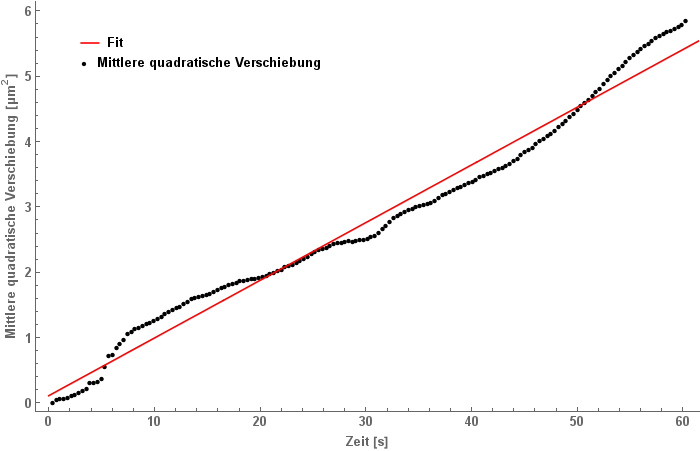
\includegraphics[width=0.9\textwidth]{msd.png}\\
		\footnotesize\sffamily\textbf{Quelle:} Selbst gezeichnet
	\end{tabular}
	\caption{Mittlere quadratische Verschiebung als Funktion der Zeit}
    \label{fig:msd}
\end{figure}
Im obigen Schaubild erkennt man einen zeitlich guten linearen Verlauf der mittleren quadratischen Verschiebung. Die Sprünge, die im Schaubild manchmal zu sehen sind, lassen sich damit erklären, dass zu den entsprechenden Zeiten weniger Messdaten zur Verfügung standen. Die (kleine) Driftbewegung der Teilchen oder eventuell äußere Störfaktoren spielen bei der Verschiebung auch eine Rolle.
\subsection{Maximale Fangkraft}
Die maximale Fangkraft $F_T$ lässt sich aus Gleichung \ref{eq:fangkraft} auf Seite \pageref{eq:fangkraft} bestimmen:
\begin{equation*}
F_T=6 \pi \eta a v_{max}
\end{equation*}
Für die Viskosität $\eta$ gilt laut Gleichung \ref{eq:diffusionskonstante} auf Seite \pageref{eq:diffusionskonstante}:
\begin{equation*}
\eta=\frac{k_B T}{6 \pi D a}
\end{equation*}
Setzt man sie in die Gleichung der Fangkraft, so ergibt sich:
\begin{equation*}
F_T=\frac{k_B \cdot v_{max} \cdot T}{D}
\end{equation*}
Dabei ist $v_{max}=\unit[6 \cdot 10^{-5}]{\frac{m}{s}}$ die experimentell bestimmte maximale Geschwindigkeit, mit der Kügelchen mit der Pinzette bewegt werden können und $k_B=\unit[1.3806 \cdot 10^{-23}]{\frac{J}{K}}$ die Boltzmann-Konstante. Die Temperatur $T$ der Flüssigkeit wurde nicht gemessen, wir werden sie jedoch mit $T=\unit[20]{^\circ C}=\unit[293]{K}$ annehmen.\\ \\
Die unbekannte Diffusionskonstante berechnen wir aus Gleichung \ref{eq:dmsDiffusion} auf Seite \pageref{eq:dmsDiffusion}:
\begin{equation*}
\langle r^2(t) \rangle=4Dt
\end{equation*}
Da wir im Abschnitt \ref{subsec:brown} die mittlere quadratische Verschiebung gegen die Zeit auftrugen, können wir aus der Steigung $m$ der gefitteten Gerade die Diffusionskonstante $D$ berechnen, denn es gilt:
\begin{equation*}
m=4D \quad \Rightarrow \quad D=\frac{m}{4}
\end{equation*}
Die Steigung des Fits betrug $m=\unit[0.088]{\frac{(\mu m)^2}{s}}$, also beträgt die Diffusionskonstante $D$:
\begin{equation*}
D=\frac{m}{4}=\frac{\unit[0.088]{\frac{(\mu m)^2}{s}}}{4}=\unit[0.022]{\frac{(\mu m)^2}{s}}=\unit[2.2 \cdot 10^{-14}]{\frac{m^2}{s}}
\end{equation*}
Durch Einsetzen der Werte erhält man die gesuchte maximale Fangkraft $F_T$:
\begin{equation}
\boxed{F_T=\frac{\unit[1.3806 \cdot 10^{-23}]{\frac{J}{K}} \cdot \unit[6 \cdot 10^{-5}]{\frac{m}{s}} \cdot \unit[293]{K}}{\unit[2.2 \cdot 10^{-14}]{\frac{m^2}{s}}}=\unit[1.1032 \cdot 10^{-14}]{N}}
\end{equation}
\subsection{Wahrscheinlichkeitsverteilung der Aufenthaltsorte der Teilchen}
Wir nahmen, wie bereits in der Versuchsdurchführung erläutert, die $(x,y)$-Koordinaten eines freien und eines mit der Pinzette gefangenen Teilches für mindestens 200 Bilder aus der Videoaufnahme auf. Diese Koordinaten plotteten wir jeweils in den Schaubildern \ref{fig:frei} und \ref{fig:fest}.
\begin{figure}[H]
\centering
\begin{subfigure}{.5\textwidth}
  \centering
  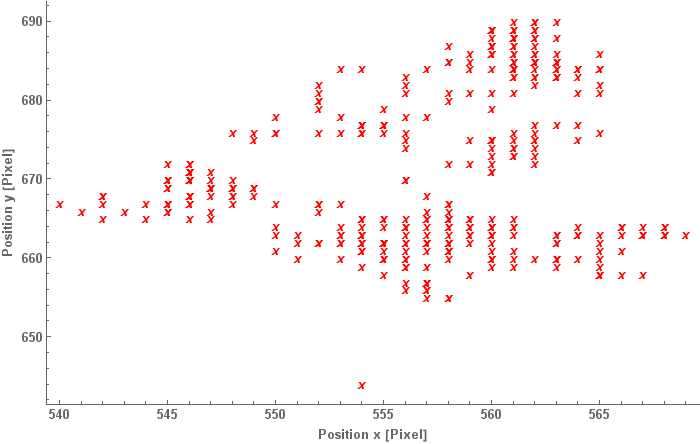
\includegraphics[width=.95\linewidth]{frei.png}
  \caption{Freies Teilchen}
  \label{fig:frei}
\end{subfigure}%
\begin{subfigure}{.5\textwidth}
  \centering
  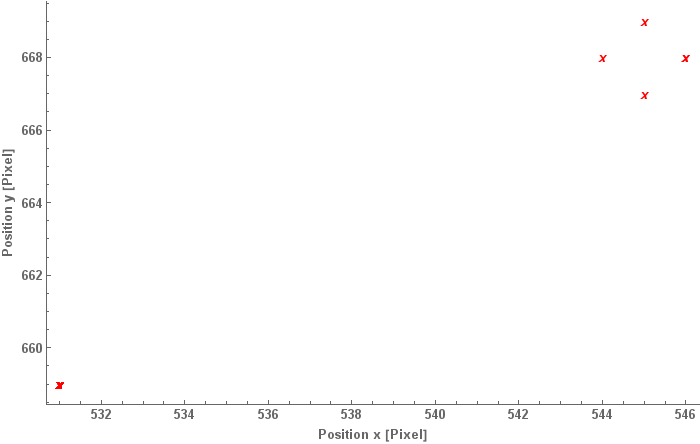
\includegraphics[width=.95\linewidth]{fest.png}
  \caption{Gefangenes Teilchen}
  \label{fig:fest}
\end{subfigure}
\caption{Koordinaten des freien und gefangenen Teilchens in Pixel}
\label{fig:koordinaten}
\end{figure}
Die beiden obigen Diagramme sind unterschiedlich skaliert, die $x$- und $y$-Bereiche sind für das gefangene Teilchen kleiner. Bei über 500 ausgewerteten Bildern sind die Aufenthaltsorte des gefangenen Teilches auf 5 Orte beschränkt. Dagegen ist die Verteilung des freien Teilchens wesentlich breiter, obwohl wir dafür 370 Bildern auswerteten. Das war zu erwarten, denn während das freie Teilchen unverhindert Brownsche Bewegungen ausführen kann, sitzt das gefangene Teilchen in der optischen Falle der Pinzette. Bewegt sie sich spontan, wird sie durch die optischen Kräfte des Laserstrahls wieder zurück in die Position der Falle gebracht.\\ \\
Weiter untersuchten wir wie oft das feste und das gefangene Teilchen entlang der $x$- und $y$-Achsen sich bewegten. Aus den Koordinaten der Aufenthaltsorten $(x(t_i),y(t_i))$ der Teilchen für jeden Zeitpunkt $t_i$ der Aufnahme berechneten wir die Verschiebung in einem Dimension entlang der $x$- und $y$-Achsen aus Gleichung \ref{eq:verschiebungEinfach} auf Seite \pageref{eq:verschiebungEinfach}:
\begin{align*}
r_x(t_i)&=x(t_i)-x(t_{i-1})\\
r_y(t_i)&=y(t_i)-y(t_{i-1})
\end{align*}
Diese Ergebnisse stellten wir in den Histogrammen \ref{fig:dmsx} und \ref{fig:dmsy} dar.
\begin{figure}[H]
\centering
\begin{subfigure}{.5\textwidth}
  \centering
  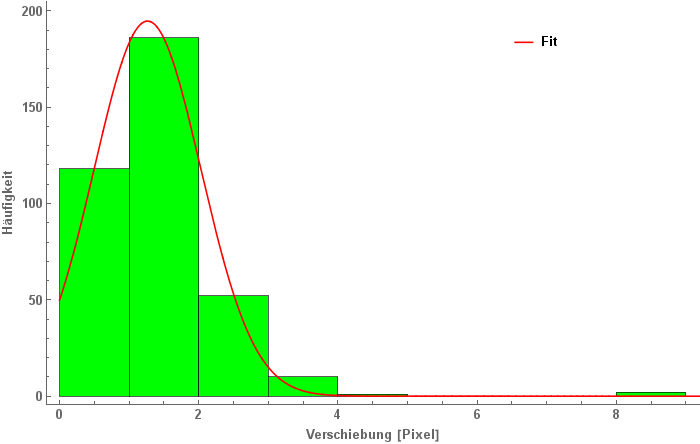
\includegraphics[width=.95\linewidth]{frei-x-dms.png}
  \caption{Freies Teilchen}
  \label{fig:dmsxfrei}
\end{subfigure}%
\begin{subfigure}{.5\textwidth}
  \centering
  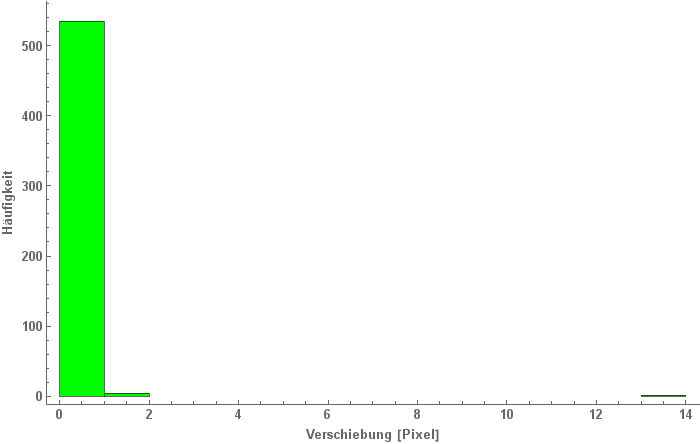
\includegraphics[width=.95\linewidth]{fest-x-dms.png}
  \caption{Gefangenes Teilchen}
  \label{fig:dmsxfest}
\end{subfigure}
\caption{Häufigkeiten der Verschiebungen der Teilchen entlang der $x$-Achse}
\label{fig:dmsx}
\end{figure}
Man erkennt an den obigen Bildern, dass das freie Teilchen entlang der $x$-Achse Verschiebungen unterschiedlicher Beträge ausführt. Die Verteilung der Verschiebungsbeträge für das gefangene Teilchen ist dagegen nicht so breit. Wir führten Histogramm-Fits der Boltzmann-Verteilungsfunktion durch. Die gefittete Funktion war:
\begin{equation}
\label{eq:fitfn}
P(x)=a \cdot e^{-b \cdot (x-c)^2}
\end{equation}
und entspricht der Maxwell-Boltzmann-Verteilungsfunktion. Der Fit war nur für das freie Teilchen sinnvoll mit folgenden Parametern:
\begin{align*}
a&=\unit[194.59]{px}\\
b&=\unit[-0.85]{\frac{1}{px^2}}\\
c&=\unit[-1.27]{px}\\
\end{align*}
Trotzdem ist in den Histogrammen \ref{fig:dmsxfrei} und \ref{fig:dmsxfest} anhand der Balken eine Boltzmann-Verteilung ersichtlich.
\begin{figure}[H]
\centering
\begin{subfigure}{.5\textwidth}
  \centering
  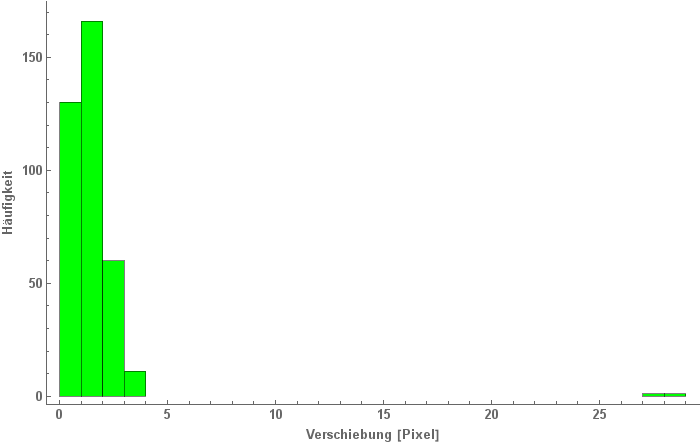
\includegraphics[width=.95\linewidth]{frei-y-dms.png}
  \caption{Freies Teilchen}
  \label{fig:dmsyfrei}
\end{subfigure}%
\begin{subfigure}{.5\textwidth}
  \centering
  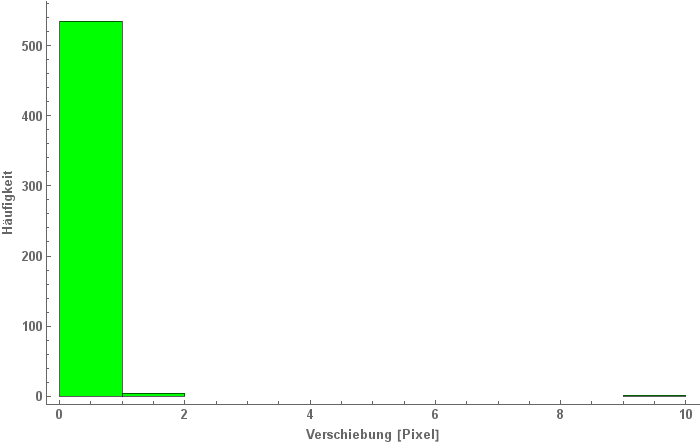
\includegraphics[width=.95\linewidth]{fest-y-dms.png}
  \caption{Gefangenes Teilchen}
  \label{fig:dmsyfest}
\end{subfigure}
\caption{Häufigkeiten der Verschiebungen der Teilchen entlang $y$-Achse}
\label{fig:dmsy}
\end{figure}
Das obige Vorgehen wiederholten wir auch für die Verschiebungen entlang der $y$-Achse für beide Teilchen (Histogramme \ref{fig:dmsyfrei} und \ref{fig:dmsyfrei}). Das freie Teilchen führt Bewegungen mit einer größere Breite an Beträgen als das gefangene aus. Leider konnte mit Mathematica die Funktion aus \ref{eq:fitfn} an keinem der Histogramme gefittet werden. Das Muster der Boltzmann-Verteilungsfunktion ist jedoch in beiden Histogrammen erkennbar.
\section{Diskussion der Ergebnisse}
In diesem Versuch untersuchten wir wie Polystyren-Kügelchen mit der optischen Pinzette eingefangen und bewegt wurden. Die Kügelchen befanden sich dabei in einer Wasserlösung, da dies Voraussetzung für die Entstehung der optischen Kräfte durch den Druck der Laserstrahlung ist.\\ \\
Weiter wurde die Brownsche Bewegung der Kolloiden in Wasser analysiert. Die Analyse erfolgte anhand der mittleren quadratischen Verschiebung, die für 170 unterschiedlichen Zeiten berechnet und aufgetragen wurde. In der Brownschen Bewegung nimmt die mittlere quadratische Verschiebung mit der Zeit linear zu, was durch unser Diagramm, trotz einer kleinen vorhanden Driftgeschwindigkeit, sehr gut bestätigt werden konnte.\\ \\
Die maximale Fangkraft, mit der Kolloide durch die Pinzette bewegt werden könnten ohne sich von der optischen Falle zu lösen, wurde auch bestimmt. Über die Qualität dieses Werts können wir keine Aussage treffen, da wir keinen theoretischen Wert bestimmt hatten oder uns bekannt war.\\ \\
Zuletzt wurde die durch die Theorie bekannte Eigenschaft der Brownschen Bewegung bestätigt, dass sie einer statistischen Boltzmann-Verteilung unterliegt. Es wurden ein freies und ein gefangenes Teilchen untersucht. Beide führten Brownsche Bewegungen durch, die Bewegungsfreiheit des gefangenen Teilchens war erwartungsgemäß sehr eingeschränkt, was durch die Gegenüberstellung deren Aufenthaltskoordinaten zu verschiedenen Zeiten klar deutlich wurde.\\ \\
Wir konnten auch untersuchen, welchen Effekt der Laserstrahl der optischen Pinzette auf schwarze und rote Farbmolekülen in Ethanollösung hatte. Während der Strahl bei roten Molekülen die Farbe aufgrund der Reflektion bekräftigte, wirkte er bei den schwarzen Farbmolekülen destruktiv.
\bibliographystyle{acm}
\bibliography{literatur}

\end{document}